\documentclass[11pt]{article}
\usepackage{amsmath, amssymb, enumerate, mathtools, dsfont, MnSymbol, tikz}
\usepackage{algorithm}
\usepackage[noend]{algpseudocode}

\begin{document}


{\bfseries Section 1.1.2}

\begin{enumerate}[1.]
    \item %1 
        graph $g$ of order $n$ with maximal number of edges if the complete graph
        $k_n$, which has $\binom{n}{2} = \frac{n(n-1)}{2}$ edges.
    \item %2
        To show a contradiction, suppose otherwise. We know there are an even 
        number of odd degree vertices, implying that there can be no odd 
        degree vertices. But the max degree of a graph is n-1 (connected to 
        every other vertex), so the degree is between 0 and n-1. Excluding 
        the odd degrees, there are not enough unique numbers to cover all the
        vertices.
    \item %3
        For later
    \item %4  
        If no such path exists, the two odd vertics are on separate connected 
        components A and B. Consider A by itself, it is a connected graph, 
        but it has an odd number of vertices with an odd degree, a contradiction
        . 
    \item %5
        Consider the following algorithm
        \begin{algorithm}
            \caption{Random Traversal}
        \begin{algorithmic}[1]
        \State i = 0
        \State v = random vertex in G
        \Repeat
        \State Mark v with i
        \State v = some vertex in N(v) that isn't marked
        \State i += 1
        \Until{all vertices in $N(v)$ is marked}
        \end{algorithmic}
        \end{algorithm}
        \begin{enumerate}[a)]
            \item Consider the vertex $v$ that we end up after running this 
                algorithm on $G$. The algorithm must have visited all vertices in
                $N(v)$, and are marked with a number. We have a path from the 
                lowest marked $u \in N(v)$ to $v$, and since $\delta(G) \geq k$, 
                this path is of length at least $k$. 
            \item 
                Once again consider the path from the lowest marked $u
                \in N(v)$ to $v$. This path in addition to the edge $uv$ 
                creates a cycle, and by above the path is at least $k$ long, 
                including $uv$ the cycle is at least $k+1$ long.
        \end{enumerate}
    \item %6
        We prove this by induction on the length of the odd closed walk. 

        Base Case: The length 3 odd closed walk is just a length 3 cycle.

        Suppose odd closed walks with lengths up to 2n - 1 contain odd cycles.
        Let $W$ = $v_1$, $v_2$, ..., $v_{2n+1} = v_1$ be a length $2n+1$ closed walk. 
        If no vertices in the walk repeat, then we are done, the odd walk is an
        odd cycle. Otherwise, let $l$ be the smallest number not $1$ such that $v_l$ 
        repeats, and let $v_l = v_k$ where $l < k$. Then we have two closed walks 
        in $W$, $v_1$, ..., $v_l = v_k$, ..., $v_{2n+1} = v_1$ and $v_l$, ..., $v_k = v_l$. The lengths of these two walks must add up to $2n+1$, thus one of them must be an odd length closed walk, which by the inductive hypothesis
        must contain an odd length cycle. 

    \item %7
        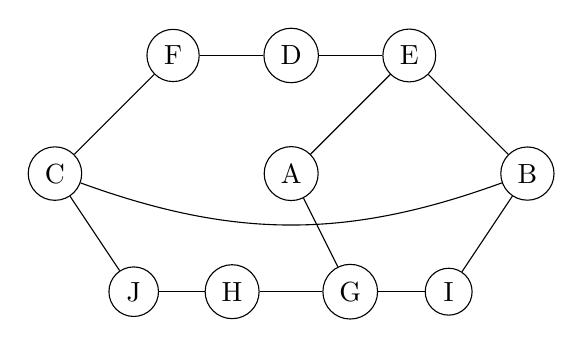
\begin{tikzpicture}
            \node[shape=circle,draw=black] (A) at (0,0) {A};
            \node[shape=circle,draw=black] (B) at (3,0) {B};
            \node[shape=circle,draw=black] (C) at (-3,0) {C};
            \node[shape=circle,draw=black] (D) at (0,1.5) {D};
            \node[shape=circle,draw=black] (E) at (1.5,1.5) {E};
            \node[shape=circle,draw=black] (F) at (-1.5,1.5) {F};
            \node[shape=circle,draw=black] (G) at (0.75,-1.5) {G};
            \node[shape=circle,draw=black] (H) at (-0.75,-1.5) {H};
            \node[shape=circle,draw=black] (I) at (2,-1.5) {I};
            \node[shape=circle,draw=black] (J) at (-2,-1.5) {J};

            \path [-] (F) edge (D);
            \path [-] (D) edge (E);
            \path [-] (E) edge (B);
            \path [-] (B) edge (I);
            \path [-] (I) edge (G);
            \path [-] (G) edge (H);
            \path [-] (H) edge (J);
            \path [-] (J) edge (C);
            \path [-] (C) edge (F);

            \path [-] (A) edge (E);
            \path [-] (A) edge (G);
            \path [-] (C) edge[bend right=20] (B);
        \end{tikzpicture}


    \item %8
        Let $P_1 = v_1, v_2, ..., v_n$ and $P_2 = u_1, u_2, ..., u_n$. Since the graph is
        connected, there exists a path $P_c = w_1 (= u_1), ..., w_m (= v_1)$ between 
        $u_1$ and $v_1$. Consider $v_i = w_{i'}$ where $i'$ is the lowest index such that
        $w_{i'} \in P_2$, and $w_{j'} = u_j$ where $j'$ is the largest index such that
        $j < i$ and $w_{j'} \in P_1$. Notice that once excluding the first and last vertices, 
        the path $w_{j'}, ..., w_{i'}$ does not contain vertices in $P_1$ and $P_2$. Let
        $P_{1-max}$ the larger of $v_1, ..., v_i$ and $v_i, ..., v_n$, likewise 
        $P_{2-max}$ the larger of $u_1, ..., u_j$ and $u_j, ..., u_n$. Since for
        $n = k_1 + k_2 = p_1 + p_2$, we have $n \leq max(k_1, k_2) + max(p_1, p_2)$, the 
        path $P_{1-max} + P_{2-max} + v_i, ..., v_j$ is longer than $P_1$ and $P_2$, which
        is a contradiction.

    \item %9
        My guess is that it is a complete graph $K_n$ with every edge to a single 
        vertex missing, which has $\binom{n-1}{2} = \frac{(n-2)(n-1)}{2}$ edges. 

    \item %10
        Using induction we prove the the minimum number of edges needed to have 
        a connected graph is $n - 1$ (a tree). 

        Base Case: $K_1$ has $0$ edges (certainly the minimum number), and is connected.

        Suppose $G$ of order $n$ requires minimum ${n - 1}$ edges to be connected.
        Consider such a connected graph with $n - 1$ edges, and consider $G + {v}$,
        $G$ with an additional vertex. If we add no edges, then the new graph is 
        disconnected, so we must add one edge. Since $G$ is connected by the inductive
        hypothesis, adding an edge between any $u \in G$ and $v$ will make $G + {v}$ 
        connected, since for $ux$ path where $x \in G$, the path $+v$ is $vx$ path.

    \item %11
        $\Rightarrow$ Suppose $e = uv$ is a bridge of $G$ and consider $G-e$. Since
        $e$ is a bridge, $G-e$ is disconnected, i.e. no $uv$ path exists in $G-e$,
        implying that $e$ is not part of any cycle in $G$. 


        $\Leftarrow$ Suppose $e = uv$ is not a bridge. Then $G - e$ is still connected, 
        i.e. there exists a $uv$ path. This path $+ e$ is a cycle.

    \item %12
        \begin{enumerate}[a)]
            \item
            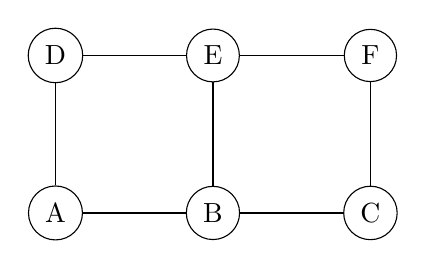
\begin{tikzpicture}
                \node[shape=circle,draw=black] (A) at (0,0) {A};
                \node[shape=circle,draw=black] (B) at (2,0) {B};
                \node[shape=circle,draw=black] (C) at (4,0) {C};
                \node[shape=circle,draw=black] (D) at (0,2) {D};
                \node[shape=circle,draw=black] (E) at (2,2) {E};
                \node[shape=circle,draw=black] (F) at (4,2) {F};

                \path [-] (A) edge (B);
                \path [-] (B) edge (C);
                \path [-] (D) edge (E);
                \path [-] (E) edge (F);
                \path [-] (A) edge (D);
                \path [-] (B) edge (E);
                \path [-] (C) edge (F);
            \end{tikzpicture} 

                This graph has no bridges and has more than one cycle.
            \item 
                We give a counter example of the contrapositive. 

            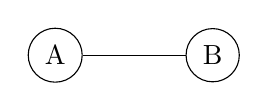
\begin{tikzpicture}
                \node[shape=circle,draw=black] (A) at (0,0) {A};
                \node[shape=circle,draw=black] (B) at (2,0) {B};

                \path [-] (A) edge (B);
            \end{tikzpicture}
                
                This graph has a bridge, but no cut vertex. 

            \item
                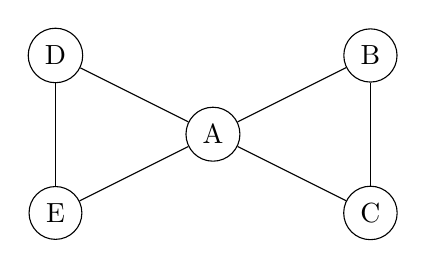
\begin{tikzpicture}
                \node[shape=circle,draw=black] (A) at (0,0) {A};
                \node[shape=circle,draw=black] (B) at (2,1) {B};
                \node[shape=circle,draw=black] (C) at (2,-1) {C};
                \node[shape=circle,draw=black] (D) at (-2,1) {D};
                \node[shape=circle,draw=black] (E) at (-2,-1) {E};

                \path [-] (A) edge (B);
                \path [-] (A) edge (C);
                \path [-] (B) edge (C);
                \path [-] (A) edge (D);
                \path [-] (A) edge (E);
                \path [-] (E) edge (D);
                \end{tikzpicture}

                This graph has no bridges and has $A$ as a cut vertex.
        \end{enumerate}

    \item %13
        Consider the graph shown in 12a. It is connected, and every vertex is part of 
        one cycle, but is not 2-connected since deleting $A$ create more connected 
        components.
    \item %14
        Suppose $G$ has no cycles and is connected. Consider $v \in V$ such that 
        $deg(v) > 1$ and $x,y \in N(v)$. Graph $G - \{v\}$ is disconnected since 
        no $xy$ path exists since if there was, this path in addition to 
        path $x$, $v$, $y$ would form a cycle in $G$. If $order = 2$, the graph does 
        not have a cycle. 
    \item %15
        \begin{enumerate}[a)]
            \item
                Consider $v \in G$ such that $\delta(G) = |N(v)|$. Then 
                $G - N(v)$ is a disconnected graph, thus $\kappa(G) \leq \delta(G)$.
            \item
                For $\delta(G) = n - 1$, this is true by definition. \newline
                Suppose $\delta(G) = n - 2$. Observe that every vertex is 
                connected to at least all but one other vertex in the graph.
                We want to show that deleting any $n-3$ nodes of $G$ still results
                in a connected graph. Consider $G$ with any $n-3$ nodes deleted, 
                we refer to the remaining three as $0, 1, 2$. Since $\delta(G) =
                n - 2$, $0$ is connected to at least one other node, say $1$. By
                the same reasoning, $2$ must be connected to at least one other 
                node, which has to be either $0$ or $1$. in either case, $0$, $1$
                and $2$ are connected. 

        \end{enumerate}

    \item %16
        \begin{enumerate}[a)]
            \item
                Suppose $\delta(G) \geq \frac{n-1}{2}$ but $G$ was not connected.
                Then it must have more than one connected component. The smallest
                connected component has $\leq n/2$ vertices, implying that 
                $\delta(G) < \frac{n-1}{2}$, a contradiction. 
            \item
            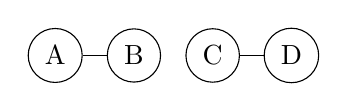
\begin{tikzpicture}
                \node[shape=circle,draw=black] (A) at (0,0) {A};
                \node[shape=circle,draw=black] (B) at (1,0) {B};
                \node[shape=circle,draw=black] (C) at (2,0) {C};
                \node[shape=circle,draw=black] (D) at (3,0) {D};

                \path [-] (A) edge (B);
                \path [-] (C) edge (D);
            \end{tikzpicture}

            $|V(G)| = 4$, $\delta(G) = 1 \geq \frac{4 - 2}{2} = 1$ and $G$ is 
            not connected. 
        \end{enumerate}

\end{enumerate}
\end{document}
